\section{Supplementary RAG allocation and resource diagnostics}
\label{sec:supp-allocation-diagnostics}
These displays retain the complete paired selection ablation, the
quality--cost tradeoff against AgentUCT-NextC, a saved allocation decision,
physical execution accounting and configuration identities. They supplement
the primary budget and task comparisons in the main paper. Five paired
search seeds, sample SDs and all endpoint identities are retained. Reused
measurements across budgets remain correlated.

The original four-MCTS 32M table separates full optimization bills from
budget-retained evaluation counts. AgentUCT's higher test F1 coexists with
lower full-bill utility than AgentUCT-NextC; no endpoint was selected by J.
The same cache and execution protocol was available to every trial, with
private caches and distinct histories.

\begin{table}[t]
\centering\small
\setlength{\tabcolsep}{2.5pt}
\caption{Five-seed results at a 32M search budget. F1 is validation-selected
primary test performance (mean $\pm$ sample SD across five seeds). $C_{\mathrm{opt}}$ is the full optimization bill in
M weighted-token units; $N_B$ counts complete evaluations retained at the
cutoff. $\Delta J$ is relative to paired MCTS-UCT runs.}
\label{tab:stage-results}
\begin{tabular}{lrrrr}
\toprule
Method & F1 (\%) $\uparrow$ & $C_{\mathrm{opt}}$ & $N_B$ & $\Delta J$\\
\midrule
AgentUCT & $\mathbf{69.57}\pm0.28$ & 59.003 & 17.6 & $+0.0367$\\
MCTS-UCT & $68.01\pm1.12$ & 59.624 & 17.8 & $0$\\
AgentUCT-NextC & $68.22\pm1.96$ & 58.319 & 17.6 & $+0.0465$\\
MCTS-Random & $68.80\pm0.87$ & 59.508 & 17.8 & $+0.0119$\\
\bottomrule
\end{tabular}
\end{table}

\begin{figure*}[t]
\centering
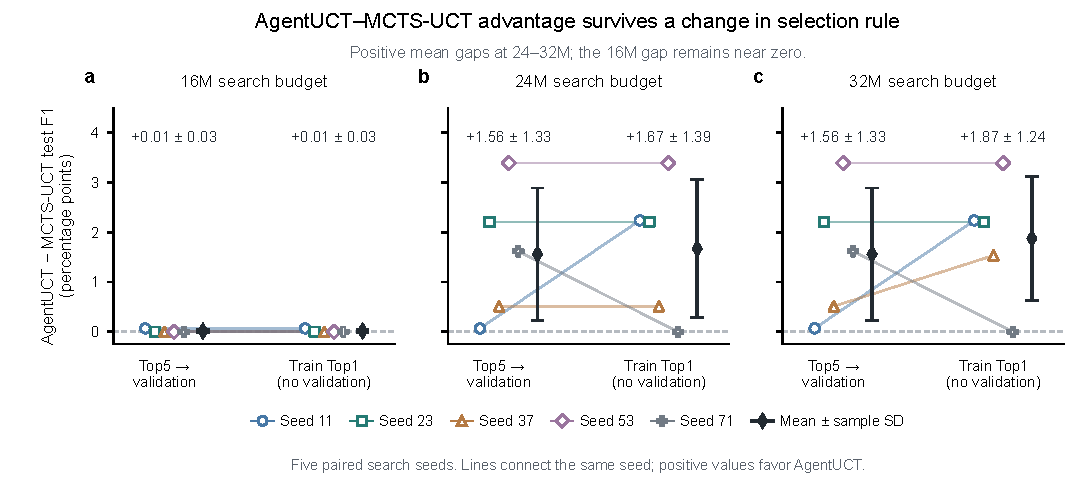
\includegraphics[width=\textwidth]{figures/top1-ablation-20261004/selection-robustness.pdf}
\caption{AgentUCT's advantage over MCTS-UCT persists without validation.
Panels compare paired test-F1 differences under both selection rules at each
budget. Symbols retain all five seeds; summaries show mean $\pm$ sample SD.
Positive values favor AgentUCT. The 16M cutoff mostly reflects initialization;
repeated endpoints across budgets reuse complete measurements.}
\label{fig:selection-robustness}
\Description{Paired AgentUCT minus MCTS-UCT test F1 at three search budgets under validation selection and direct training Top1 selection. The positive mean advantage at 24M and 32M persists under both rules.}
\end{figure*}

\begin{figure*}[t]
\centering
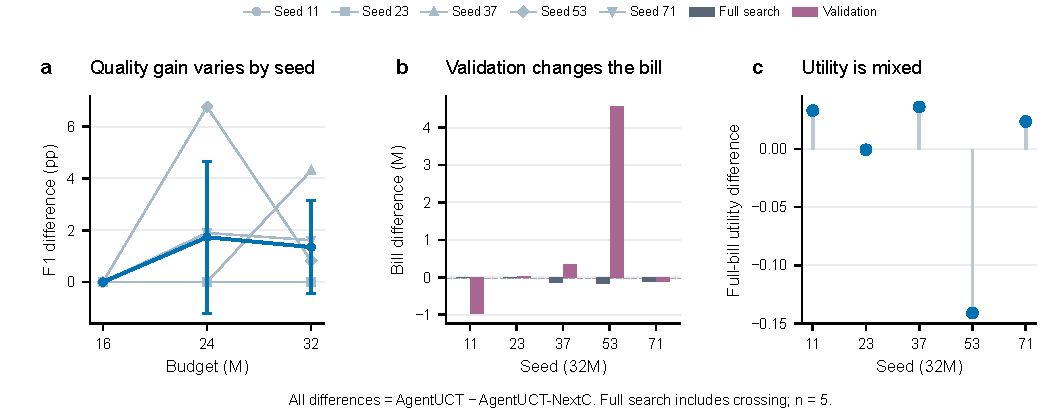
\includegraphics[width=\textwidth]{figures/rag-budget-overlay-20261004/completion-tradeoff.pdf}
\caption{Completion pricing relative to AgentUCT-NextC. (a) Paired test-F1
differences at each budget, with all five seeds and the mean $\pm$ sample SD.
(b) Actual full-search and validation-bill differences at 32M, including the
crossing evaluation in search. (c) Auxiliary full-bill utility differences for
the same five seeds. Positive quality and cost differences respectively mean
higher F1 and a higher bill; positive utility means higher $J$.}
\label{fig:completion-tradeoff}
\Description{Three panels show AgentUCT minus AgentUCT-NextC in test F1, full search and validation cost, and full-bill utility, retaining all five seeds.}
\end{figure*}

\begin{table}[t]
\centering\small\setlength{\tabcolsep}{3pt}
\caption{A saved decision at seed 53, iteration 9. Both actions have
$N=1$ and exploration bonus 2.075225. Cost is predicted remaining work in
M weighted tokens; the final index subtracts $2\widehat b/C_{\rm ref}$.}
\label{tab:completion-choice}
\begin{tabular}{lrrr}
\toprule
Query action & $Q+\mathrm{bonus}$ & Cost (M) & Final index\\
\midrule
Identity & 2.7265 & 1.7760 & 0.3112\\
Synonyms (selected) & 2.6912 & 1.0157 & 1.3100\\
\bottomrule
\end{tabular}
\end{table}

\begin{figure*}[t]
\centering
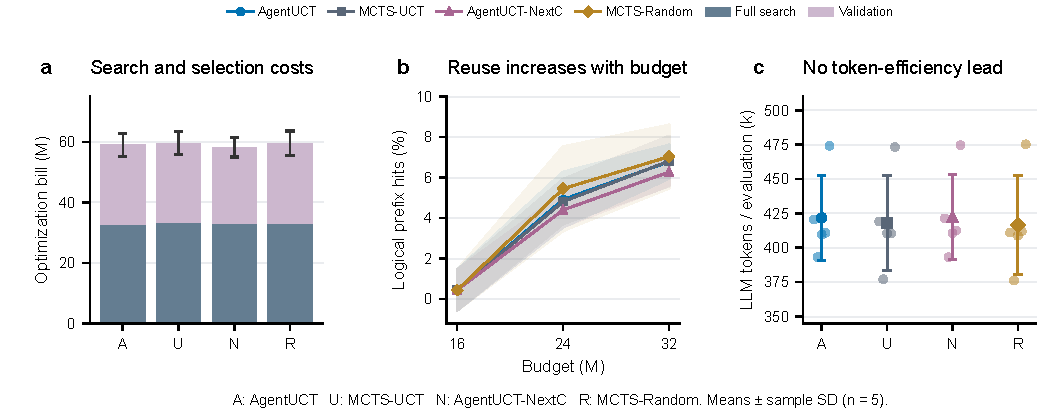
\includegraphics[width=\textwidth]{figures/rag-budget-overlay-20261004/execution-accounting.pdf}
\caption{Execution accounting for all four methods. (a) Mean full optimization
bill at 32M, separated into search and validation; error bars show the sample
SD of the total over five seeds. Test and preparation are separately reported.
(b) Logical hit fractions over all demanded prefix visits at each cutoff,
including zero-cost stages; bands show sample SD. (c) Actual unweighted LLM
input-plus-output tokens per completed evaluation at 32M, with all seeds and
mean $\pm$ sample SD. Logical hits do not measure a no-cache counterfactual.}
\label{fig:execution-accounting}
\Description{Full optimization cost is decomposed into search and validation, followed by logical prefix hit rates and physical LLM tokens per evaluation for the four algorithms.}
\end{figure*}

\begin{figure*}[t]
\centering
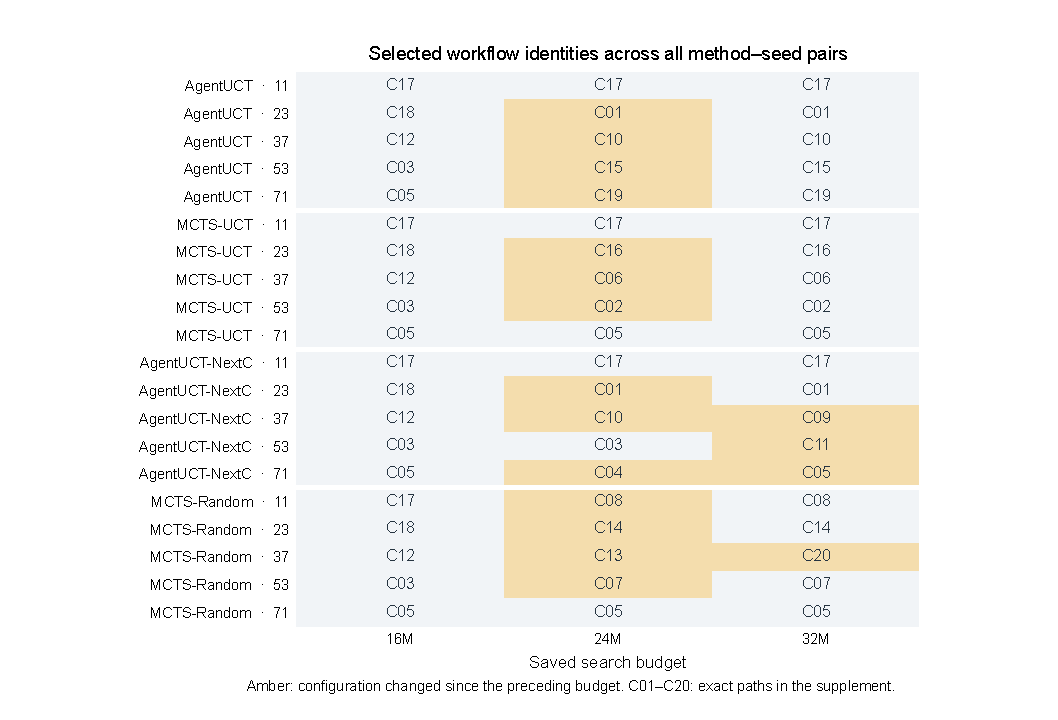
\includegraphics[width=\textwidth]{figures/rag-budget-overlay-20261004/configuration-migration.pdf}
\caption{Budget migration of validation-selected workflows. Rows retain each
method and search seed; columns use the three complete affordable snapshots.
Codes identify exact component sequences in the supplementary configuration
dictionary. Amber marks a changed configuration since the preceding budget.
Equal codes across independent runs identify the same workflow, while its
physical test execution and prediction may differ.}
\label{fig:configuration-migration}
\Description{Twenty method and seed rows show the selected configuration at 16, 24 and 32 million weighted tokens; amber marks changed configurations.}
\end{figure*}
